\documentclass{amia}
\usepackage{graphicx}
\usepackage[labelfont=bf]{caption}
\usepackage[superscript,nomove]{cite}
\usepackage{color}
\usepackage{wrapfig}

\begin{document}

\title{Creating RDF data on trauma care organizations from questionnaires}

\author{Joseph R. Utecht, BA$^{1}$, Mathias Brochhausen, PhD$^{1}$}

\institutes{
    $^1$University of Arkansas for Medical Science, Little Rock, AR, USA\\
}

\maketitle

\section*{Background}

The CAFE (Comparative Assessment Framework for Environments of Trauma Care) project (1R01GM111324) aims to address the problem of lack of comparable data about trauma care organizations (trauma systems, trauma centers) and their components.
To achieve this we created a semantically-rich vocabulary in form of an OWL ontology called OOSTT \cite{ref1}.
OOSTT will be used as the semantic backbone of a web-based IT infrastructure that allows representatives of trauma system or trauma centers to enter data about their institution and compare it in real-time to other institutions of the same type.
In order to facilitate  managing the entered data, we needed the data provided by the users in a format that allows easy integration with the OWL file.
Therefore, we decide to create data in the Resource Description Framework (RDF).
Our goal is to provide a user-friendly questionnaire that creates RDF as the users answer questions.
In this poster we describe the methodologies used to build the CAFE questionnaire and the strategies of how RDF data are created.

\section*{Methods}


The Resource Description Framework (RDF), the basic standard of the Semantic Web, allows the representation of entities and their potential relationships to many other entities
RDF data can be stored in triplestores alongside with OWL files.
The latter provide computer-interpretable definitions of the entities in  a domain, in this case of the trauma care domain, e.g trauma center, trauma program manager, etc.
The requirement of user-friendly data entry restricted the complexity of the interface used for data-entry, thus we decided on a traditional questionnaire similar to, for instance, Lime Survey. 
The application we have built uses a decoupled web interface built using the Javascript library Angular2.
As soon as a user answers a question the answer is recorded by the server, without the user needing to press a save or submit button, and the decoupled nature means that user interaction is not interrupted if the server is busy processing previous answers.
The innovation is that our survey does not only store the answer in a relational database. 
It also creates an RDF statement representing the portion of reality the answer reports.
For example, if the question is "Does your trauma center have a trauma registrar?" RDF statements are created that represent the individual trauma registrar role, its bearer, and the individual trauma center in question, specifying that the trauma registrar is an organizational member of that trauma center.
Our tool allows asking questions with boolean values, multi-selection items , drop down menus and entering date or measurement data.

\section*{Results}

\begin{wrapfigure}{r}{0.5\textwidth}
  \begin{center}
    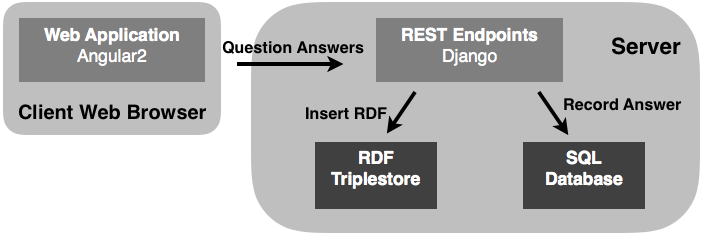
\includegraphics[width=0.48\textwidth]{pics/cafe_process2.png}
  \end{center}
  \caption{CAFE Project Process.}
  \label{cafe_process}
\end{wrapfigure}

The result of this work is the CAFE web application; the source of which is available on Github (https://github.com/cafe-trauma/). 
This site allows us to perform the mapping from question to RDF while constructing the questions for the questionnaire.
The RDF representations of questions are created one triple at a time by a non-developer through an administrative interface, and can range from a single RDF statement to a complex set of triples.
The wording, logic, and RDF mapping of questions are stored in a relational database and accessed by the front-end through a series of REST endpoints on the server.
When a user answers a question the server-side component will record the answer in the relational database and also insert the configured RDF for that question into the triplestore (Figure ~\ref{cafe_process}).
From the users point of view the questionnaire does not differ in any way from a more typical questionnaire backed by a relational database.
The benefit of this method is that our semantically enriched view of a users organization is available immediately to both build visualizations for the user and to share with public health researchers.

\makeatletter
\renewcommand{\@biblabel}[1]{\hfill #1.}
\makeatother


\bibliographystyle{unsrt}
\begin{thebibliography}{1}
\setlength\itemsep{-0.1em}

\bibitem{ref1}
Utecht J, Judkins J, Colvin T Jr., et al. OOSTT: a Resource for Analyzing the Organizational Structures of Trauma Centers and Trauma Systems. CEUR Workshop Proc. 2016 Aug;1747.

\end{thebibliography}

\end{document}
